\documentclass{standalone}
\usepackage{tikz}

\begin{document}

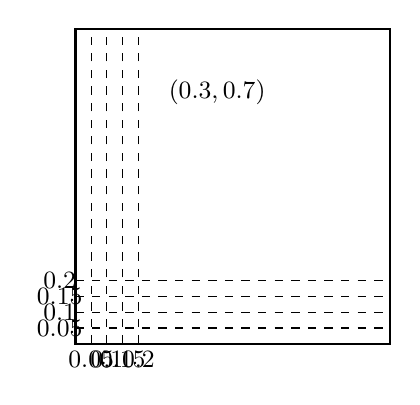
\begin{tikzpicture}[scale=4]
    % Draw the larger square frame
    \draw[thick] (0,0) rectangle (1,1);
    
    % Mark the edges of the frame with coordinates in tenths
    \foreach \x in {0.05, 0.1, 0.15, 0.2} {
        \draw[dashed] (\x,0) -- (\x,1);
        \draw[dashed] (0,\x) -- (1,\x);
        \node at (\x,-0.05) {\small $\x$};
        \node at (-0.05,\x) {\small $\x$};
    }
    
    % Draw the smaller white square representing the object
    \fill[white] (0.3, 0.7) rectangle (0.6, 0.9);
    
    % Label the position of the object
    \node at (0.45, 0.8) {\small $(0.3, 0.7)$};
\end{tikzpicture}

\end{document}